%\iffalse
\let\negmedspace\undefined
\let\negthickspace\undefined
\documentclass[journal,12pt,twocolumn]{IEEEtran}
\usepackage{cite}
\usepackage{amsmath,amssymb,amsfonts,amsthm}
\usepackage{algorithmic}
\usepackage{graphicx}
\usepackage{textcomp}
\usepackage{xcolor}
\usepackage{txfonts}
\usepackage{listings}
\usepackage{enumitem}
\usepackage{mathtools}
\usepackage{gensymb}
\usepackage{comment}
\usepackage[breaklinks=true]{hyperref}
\usepackage{tkz-euclide} 
\usepackage{listings}
\usepackage{gvv}                            \usepackage{tikz}
\usepackage{circuitikz}
\def\inputGnumericTable{}                                
\usepackage[latin1]{inputenc}                            
\usepackage{color}                      \usepackage{gensymb}
\usepackage{array}                                       
\usepackage{longtable}                                   
\usepackage{calc}                              
\usepackage{tikz}
\usepackage{multirow}                                    
\usepackage{hhline}                                      
\usepackage{ifthen}                            
\usepackage{caption}
\usepackage{lscape}
\usepackage{amsmath}
\newtheorem{theorem}{Theorem}[section]
\newtheorem{problem}{Problem}
\newtheorem{proposition}{Proposition}[section]
\newtheorem{lemma}{Lemma}[section]
\newtheorem{corollary}[theorem]{Corollary}
\newtheorem{example}{Example}[section]
\newtheorem{definition}[problem]{Definition}
\newcommand{\BEQA}{\begin{eqnarray}}
\newcommand{\EEQA}{\end{eqnarray}}
\newcommand{\define}{\stackrel{\triangle}{=}}
\theoremstyle{remark}
\newtheorem{rem}{Remark}

\begin{document}

\bibliographystyle{IEEEtran}
\vspace{3cm}

\title{GATE 2022 IN Q52}
\author{EE23BTECH11009 - AROSHISH PRADHAN$^{*}$% <-this % stops a space
}
\maketitle
\newpage
\bigskip
\textbf{Question:} In the circuit shown, the load is driven by a sinusoidal A.C. voltage source $V_1 = 100\angle0\degree V$ at $50Hz$. Given $R_1 = 20\Omega$, $C_1 = \brak{\frac{1000}{\pi}}\mu F$, $L_1 = \brak{\frac{20}{\pi}}mH$ and $R_2 = 4\Omega$, the power factor is \_\_\_\_\_ (round off to one decimal place)\\
\hfill(GATE 2022 IN Q52)
\begin{figure}[!h]
    \centering
    \begin{circuitikz}[scale = 0.8]
        \draw(0, 0) -- (1, 0);
        \draw(1, 0.5) -- (1, -0.5);
        \draw(4, 0.5) -- (4, -0.5);
        \draw(4, 0) -- (5, 0);

        \draw(1, 0.5) to[R, l = $6\Omega$](4, 0.5);
        \draw(1, -0.5) to[R, l_ = $3\Omega$](4, -0.5);

        \draw(0, 0) -- (0, -2);
        \draw(5, 0) -- (5, -2);

        \draw(0, -2) to[C, l = $1\mu F$](2, -2);
        \draw(2, -2) to [R, l = $10\Omega$](5, -2);

        \draw(0, -2) -- (0, -3.5);
        \draw(5, -2) -- (5, -3.5);

        \draw(0, -3.5) to[battery2, l_ = $10V$](1.5, -3.5);
        \draw (1.5, -3.5) to[switch, l = S] (2, -3.5);
        \draw(2, -3.5) to [R, l = $2\Omega$](5, -3.5);

        \draw[->](0, -3.5) -- (0, -2.5) node[midway, left] {$I$}; 
    \end{circuitikz}
    \caption{}
    \label{fig:1_gate.ee.22.31}
\end{figure}

\solution
\begin{table}[!h]
    \centering
    \begin{tabular}{|c|c|c|}
    \hline
       \textbf{Symbol}  & \textbf{Value} &  \textbf{Description}\\
    \hline
       $V_{in}$  &  &  Input Voltage\\
    \hline
        $V_{out}$ & & Output Voltage\\
    \hline
        $f$ & $1000Hz$ & Input Wave Frequency\\
    \hline
        $T$ & $\dfrac{1}{f} = 10^{-3} s$ & Input Wave Time Period\\
    \hline
        \multirow{4}{*}{$R$} & (a) $0.5k\Omega$ & \multirow{4}{*}{Resistance}\\
        \cline{2-2}
        & (b) $5k\Omega$ &\\
        \cline{2-2}
        & (c) $0.5k\Omega$ &\\
        \cline{2-2}
        & (d) $5k\Omega$ &\\
    \hline
        \multirow{4}{*}{$C$} & (a) $0.1\mu F$ & \multirow{4}{*}{Capacitance}\\
        \cline{2-2}
        & (b) $1\mu F$ &\\
        \cline{2-2}
        & (c) $0.1\mu F$ &\\
        \cline{2-2}
        & (d) $1\mu F$ &\\
    \hline
        $\tau$ & $RC$ & Time Constant\\
    \hline
    \end{tabular}
    \caption{Given Parameters}
    \label{tab:1_gate.23.ph.37}
\end{table}


\begin{align}
    Z_{\text{eff}} &= R_2 + j\omega L_1 + \frac{\frac{R_1}{j\omega C_1}}{R_1 + \frac{1}{j\omega C_1}}\\
    &= 4 + 2j + \frac{-200j}{20 - 10j}\\
    &= 8-6j
\end{align}
$\therefore$ Power Factor:
\begin{align}
    \cos(\phi) &= \frac{\mathrm{Re}(Z_{\text{eff}})}{\abs{Z_{\text{eff}}}}\\
    &= \frac{8}{\sqrt{8^2 + 6^2}}\\
    &= 0.8
\end{align}
\begin{figure}[!h]
    \centering
    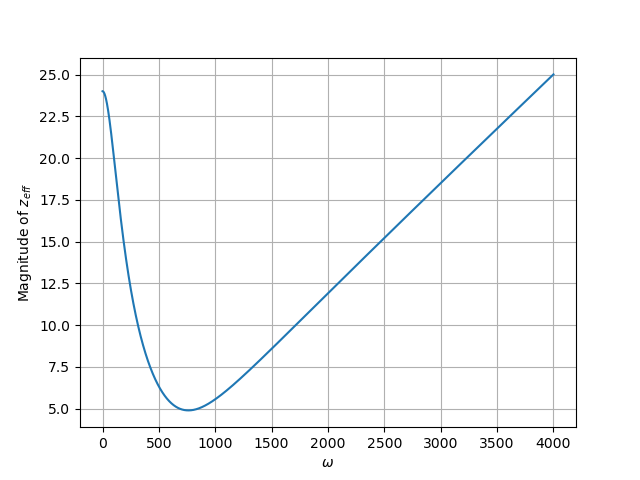
\includegraphics[width = \columnwidth]{figs/Zplot.png}
    \caption{Plot of $Z_{\text{eff}}$ vs $\omega$}
    \label{fig:2_gate.22.in.52}
\end{figure}
\end{document}

